\documentclass[letterpaper,12pt]{article}
\usepackage[margin=.65in,top=.72in,bottom=.62in,headheight=16pt,headsep=15pt,footskip=19pt]{geometry}
\usepackage[T1]{fontenc}
\usepackage{lmodern,tikz,fancyhdr}\pdfmapfile{+lm.map}
\usetikzlibrary{arrows.meta,shapes.geometric}
\pagestyle{fancy}\fancyhf{}\renewcommand{\headrulewidth}{0pt}\renewcommand{\footrulewidth}{0pt}
\setlength{\parindent}{0pt}\setlength{\parskip}{0pt}
\fancyhead[L]{\small Week 45 / The visible side / K--1}
\fancyfoot[L]{\footnotesize Bellingham Math Circle / Week 45 / W45-k-1-v2}\fancyfoot[R]{\footnotesize\thepage}
\begin{document}
\noindent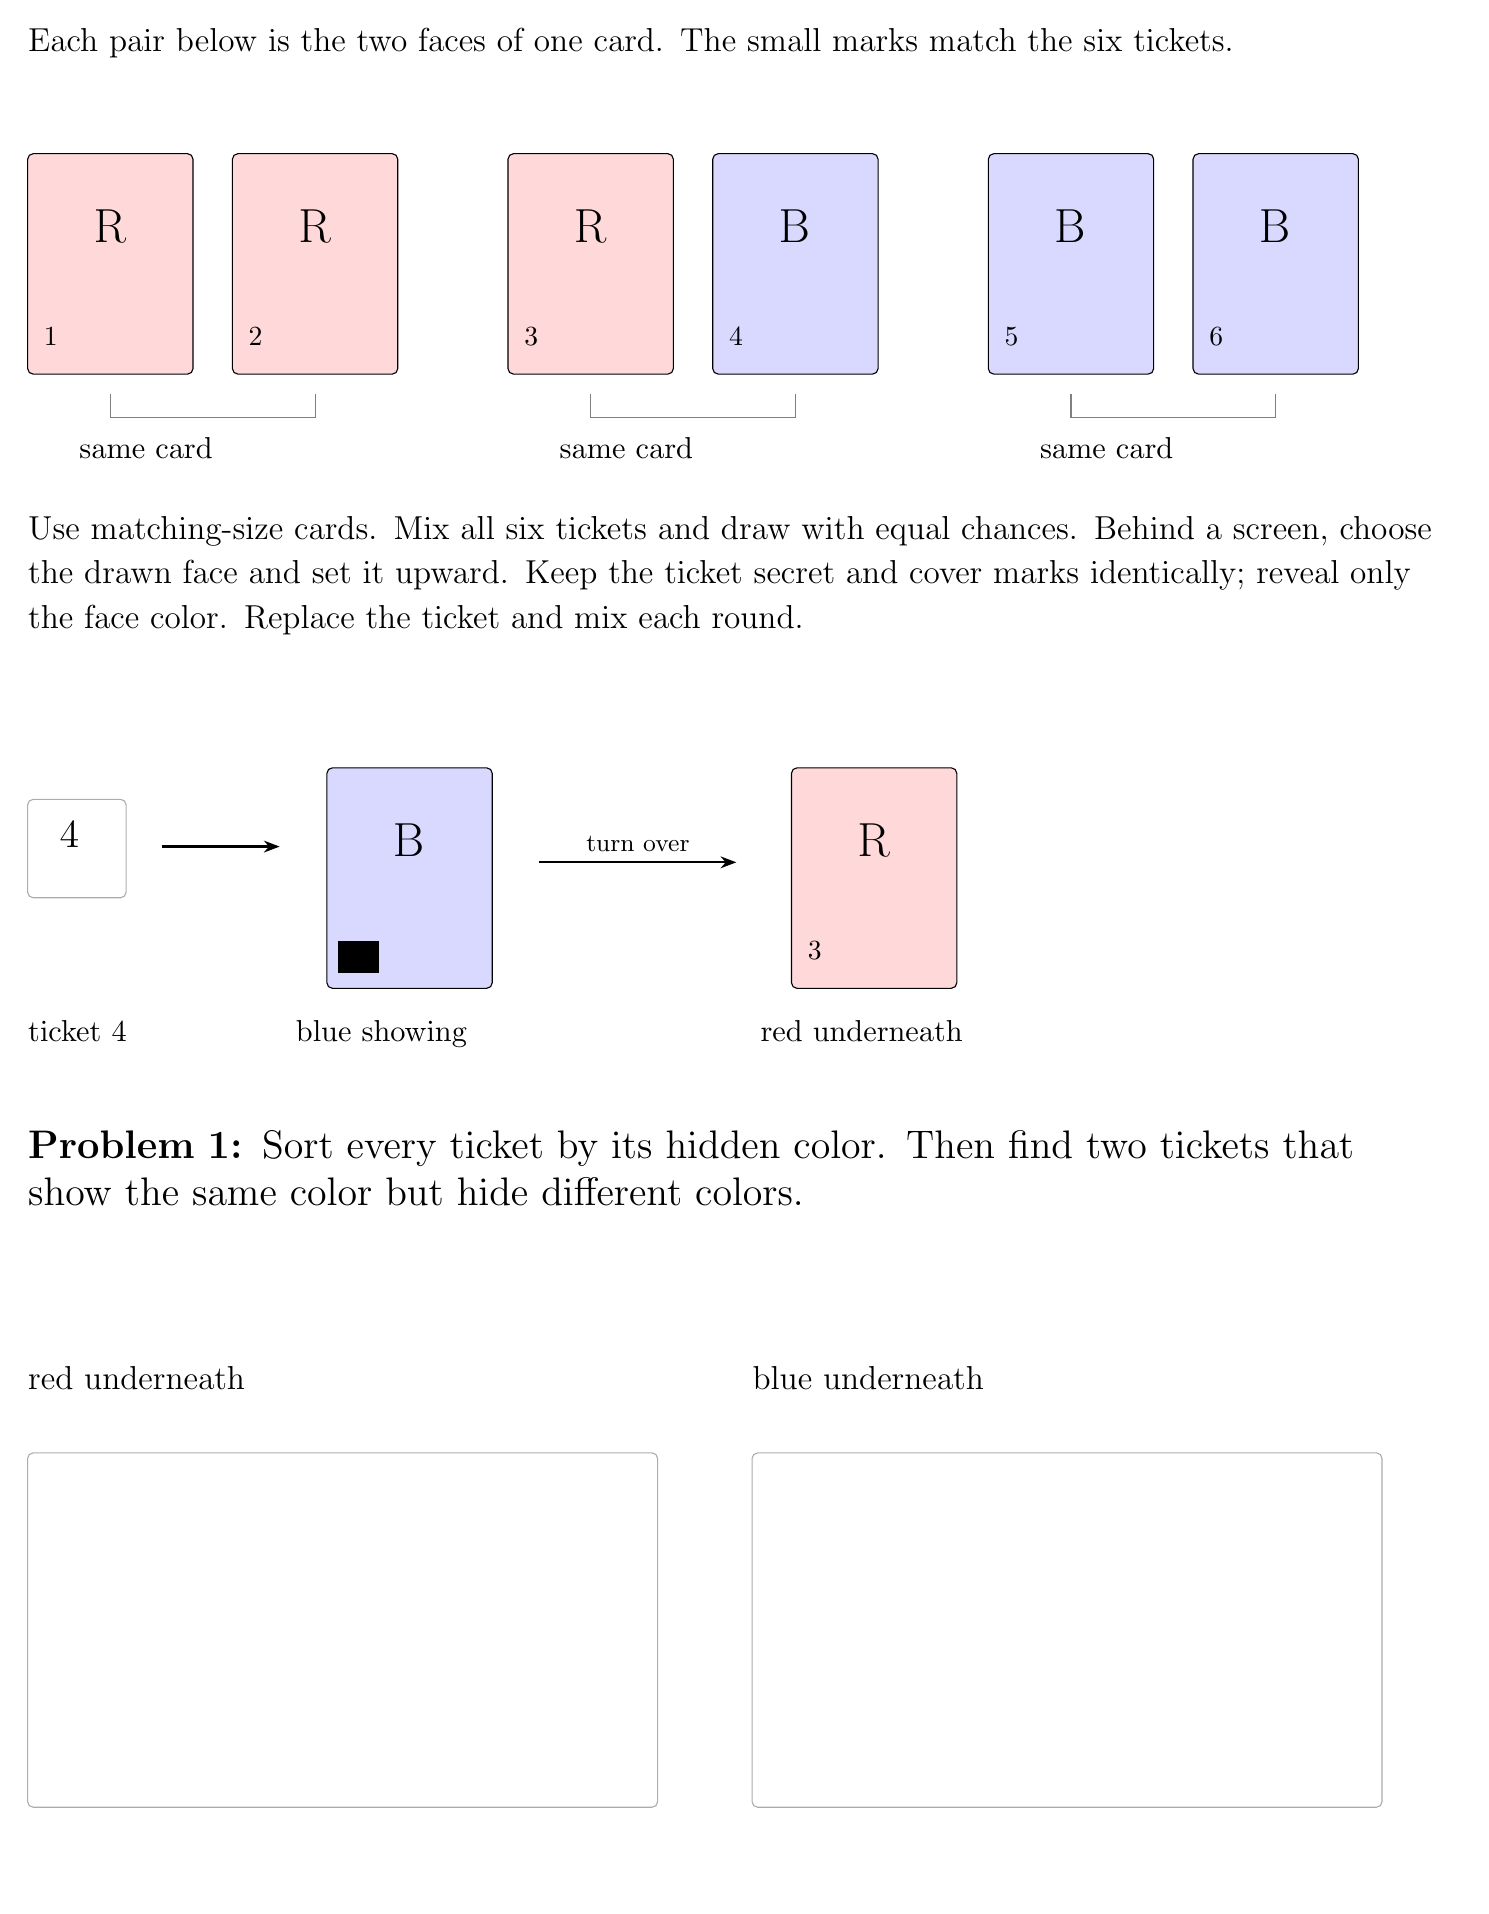
\begin{tikzpicture}[x=1cm,y=1cm]\path[use as bounding box] (0,0) rectangle (18.2,-23.6);
\node[anchor=north west,text width=18cm,inner sep=0pt,font=\fontsize{13}{16}\selectfont] at (0,0) {Each pair below is the two faces of one card. The small marks match the six tickets.};
\draw[fill=red!15,rounded corners=2pt] (0.0,-1.6) rectangle (2.1,-4.4);
\node[anchor=north west,text width=0.6cm,inner sep=0pt,font=\fontsize{17}{20}\selectfont] at (0.8300000000000001,-2.3) {R};
\node[anchor=north west,text width=0.7cm,inner sep=0pt,font=\fontsize{10}{13}\selectfont] at (0.2,-3.8000000000000003) {1};
\draw[fill=red!15,rounded corners=2pt] (2.6,-1.6) rectangle (4.7,-4.4);
\node[anchor=north west,text width=0.6cm,inner sep=0pt,font=\fontsize{17}{20}\selectfont] at (3.43,-2.3) {R};
\node[anchor=north west,text width=0.7cm,inner sep=0pt,font=\fontsize{10}{13}\selectfont] at (2.8000000000000003,-3.8000000000000003) {2};
\draw[gray] (1.05,-4.65) -- (1.05,-4.95) -- (3.65,-4.95) -- (3.65,-4.65);
\node[anchor=north west,text width=4cm,inner sep=0pt,font=\fontsize{11}{14}\selectfont] at (0.65,-5.2) {same card};
\draw[fill=red!15,rounded corners=2pt] (6.1,-1.6) rectangle (8.2,-4.4);
\node[anchor=north west,text width=0.6cm,inner sep=0pt,font=\fontsize{17}{20}\selectfont] at (6.93,-2.3) {R};
\node[anchor=north west,text width=0.7cm,inner sep=0pt,font=\fontsize{10}{13}\selectfont] at (6.3,-3.8000000000000003) {3};
\draw[fill=blue!15,rounded corners=2pt] (8.7,-1.6) rectangle (10.799999999999999,-4.4);
\node[anchor=north west,text width=0.6cm,inner sep=0pt,font=\fontsize{17}{20}\selectfont] at (9.53,-2.3) {B};
\node[anchor=north west,text width=0.7cm,inner sep=0pt,font=\fontsize{10}{13}\selectfont] at (8.899999999999999,-3.8000000000000003) {4};
\draw[gray] (7.1499999999999995,-4.65) -- (7.1499999999999995,-4.95) -- (9.75,-4.95) -- (9.75,-4.65);
\node[anchor=north west,text width=4cm,inner sep=0pt,font=\fontsize{11}{14}\selectfont] at (6.75,-5.2) {same card};
\draw[fill=blue!15,rounded corners=2pt] (12.2,-1.6) rectangle (14.299999999999999,-4.4);
\node[anchor=north west,text width=0.6cm,inner sep=0pt,font=\fontsize{17}{20}\selectfont] at (13.03,-2.3) {B};
\node[anchor=north west,text width=0.7cm,inner sep=0pt,font=\fontsize{10}{13}\selectfont] at (12.399999999999999,-3.8000000000000003) {5};
\draw[fill=blue!15,rounded corners=2pt] (14.799999999999999,-1.6) rectangle (16.9,-4.4);
\node[anchor=north west,text width=0.6cm,inner sep=0pt,font=\fontsize{17}{20}\selectfont] at (15.629999999999999,-2.3) {B};
\node[anchor=north west,text width=0.7cm,inner sep=0pt,font=\fontsize{10}{13}\selectfont] at (14.999999999999998,-3.8000000000000003) {6};
\draw[gray] (13.25,-4.65) -- (13.25,-4.95) -- (15.85,-4.95) -- (15.85,-4.65);
\node[anchor=north west,text width=4cm,inner sep=0pt,font=\fontsize{11}{14}\selectfont] at (12.85,-5.2) {same card};
\node[anchor=north west,text width=18cm,inner sep=0pt,font=\fontsize{13}{16}\selectfont] at (0,-6.2) {Use matching-size cards. Mix all six tickets and draw with equal chances. Behind a screen, choose the drawn face and set it upward. Keep the ticket secret and cover marks identically; reveal only the face color. Replace the ticket and mix each round.};
\draw[gray!65,rounded corners=2pt] (0,-9.8) rectangle (1.25,-11.05);
\node[anchor=north west,text width=0.5cm,inner sep=0pt,font=\fontsize{14}{17}\selectfont] at (0.4,-10.08) {4};
\draw[-{Stealth[length=2mm]},line width=.8pt] (1.7,-10.4) -- (3.2,-10.4) node[midway,above,font=\small] {};
\draw[fill=blue!15,rounded corners=2pt] (3.8,-9.4) rectangle (5.9,-12.2);
\node[anchor=north west,text width=0.6cm,inner sep=0pt,font=\fontsize{17}{20}\selectfont] at (4.63,-10.1) {B};
\draw[fill=black] (3.9499999999999997,-12.0) rectangle (4.45,-11.6);
\draw[-{Stealth[length=2mm]},line width=.8pt] (6.5,-10.6) -- (9,-10.6) node[midway,above,font=\small] {turn over};
\draw[fill=red!15,rounded corners=2pt] (9.7,-9.4) rectangle (11.799999999999999,-12.2);
\node[anchor=north west,text width=0.6cm,inner sep=0pt,font=\fontsize{17}{20}\selectfont] at (10.53,-10.1) {R};
\node[anchor=north west,text width=0.7cm,inner sep=0pt,font=\fontsize{10}{13}\selectfont] at (9.899999999999999,-11.6) {3};
\node[anchor=north west,text width=3cm,inner sep=0pt,font=\fontsize{11}{14}\selectfont] at (0,-12.6) {ticket 4};
\node[anchor=north west,text width=5cm,inner sep=0pt,font=\fontsize{11}{14}\selectfont] at (3.4,-12.6) {blue showing};
\node[anchor=north west,text width=7cm,inner sep=0pt,font=\fontsize{11}{14}\selectfont] at (9.3,-12.6) {red underneath};
\node[anchor=north west,text width=18cm,inner sep=0pt,font=\fontsize{14}{17}\selectfont] at (0,-14) {\textbf{Problem 1:} Sort every ticket by its hidden color. Then find two tickets that show the same color but hide different colors.};
\node[anchor=north west,text width=8cm,inner sep=0pt,font=\fontsize{13}{16}\selectfont] at (0.0,-17) {red underneath};
\draw[gray!65,rounded corners=2pt] (0.0,-18.1) rectangle (8.0,-22.6);
\node[anchor=north west,text width=8cm,inner sep=0pt,font=\fontsize{13}{16}\selectfont] at (9.2,-17) {blue underneath};
\draw[gray!65,rounded corners=2pt] (9.2,-18.1) rectangle (17.2,-22.6);
\end{tikzpicture}
\newpage
\noindent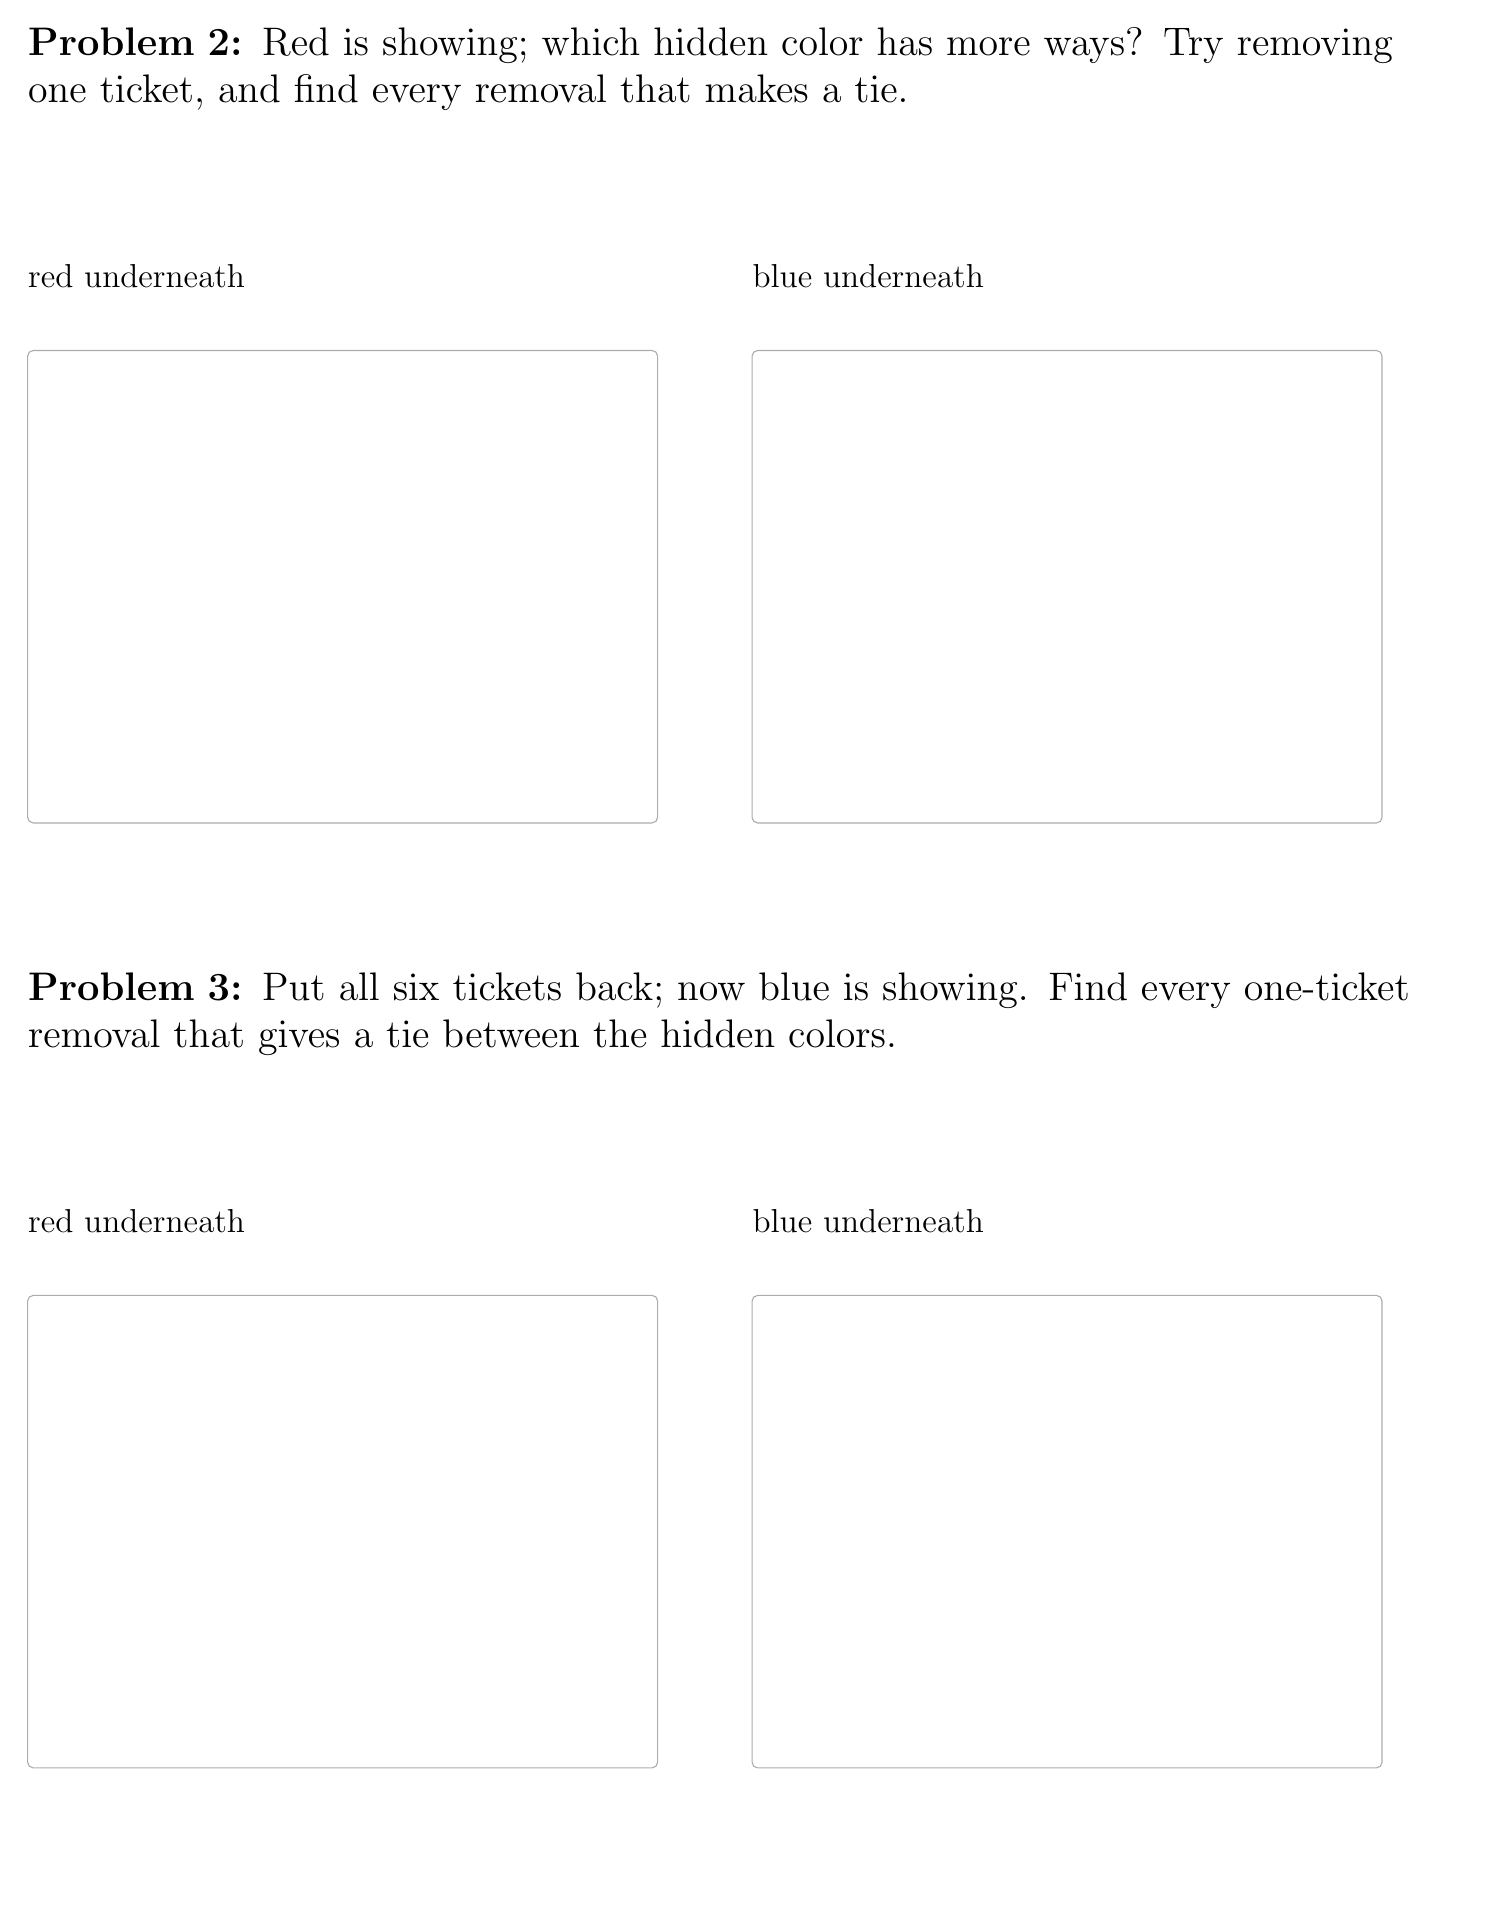
\begin{tikzpicture}[x=1cm,y=1cm]\path[use as bounding box] (0,0) rectangle (18.2,-23.6);
\node[anchor=north west,text width=18cm,inner sep=0pt,font=\fontsize{14}{17}\selectfont] at (0,0) {\textbf{Problem 2:} Red is showing; which hidden color has more ways? Try removing one ticket, and find every removal that makes a tie.};
\node[anchor=north west,text width=8cm,inner sep=0pt,font=\fontsize{13}{16}\selectfont] at (0.0,-3) {red underneath};
\draw[gray!65,rounded corners=2pt] (0.0,-4.1) rectangle (8.0,-10.1);
\node[anchor=north west,text width=8cm,inner sep=0pt,font=\fontsize{13}{16}\selectfont] at (9.2,-3) {blue underneath};
\draw[gray!65,rounded corners=2pt] (9.2,-4.1) rectangle (17.2,-10.1);
\node[anchor=north west,text width=18cm,inner sep=0pt,font=\fontsize{14}{17}\selectfont] at (0,-12) {\textbf{Problem 3:} Put all six tickets back; now blue is showing. Find every one-ticket removal that gives a tie between the hidden colors.};
\node[anchor=north west,text width=8cm,inner sep=0pt,font=\fontsize{13}{16}\selectfont] at (0.0,-15) {red underneath};
\draw[gray!65,rounded corners=2pt] (0.0,-16.1) rectangle (8.0,-22.1);
\node[anchor=north west,text width=8cm,inner sep=0pt,font=\fontsize{13}{16}\selectfont] at (9.2,-15) {blue underneath};
\draw[gray!65,rounded corners=2pt] (9.2,-16.1) rectangle (17.2,-22.1);
\end{tikzpicture}
\newpage
\noindent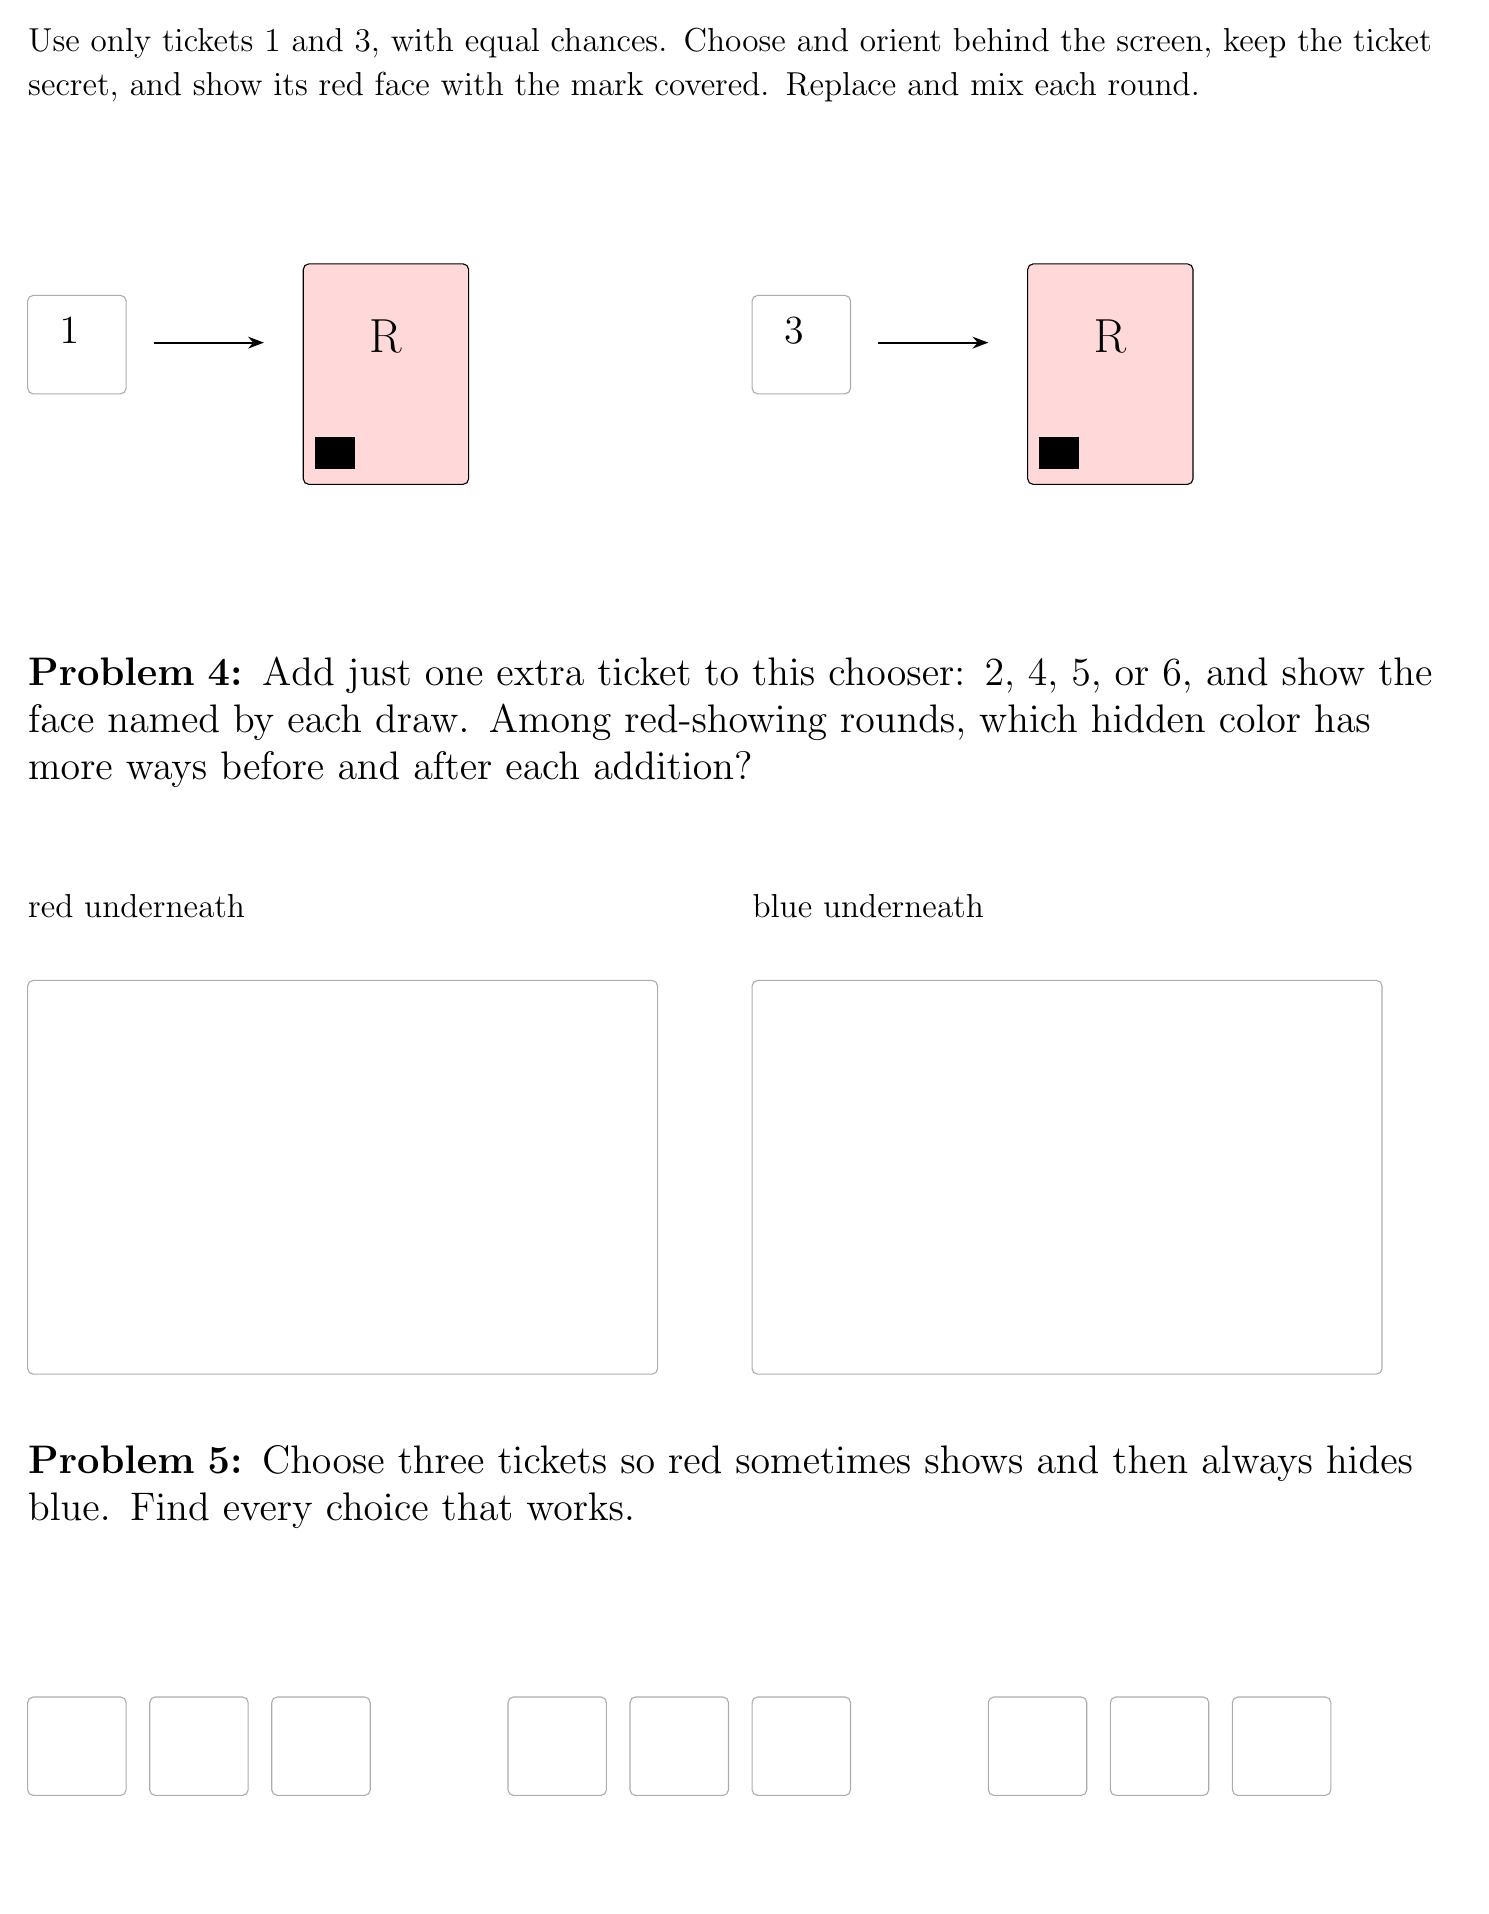
\begin{tikzpicture}[x=1cm,y=1cm]\path[use as bounding box] (0,0) rectangle (18.2,-23.6);
\node[anchor=north west,text width=18cm,inner sep=0pt,font=\fontsize{13}{16}\selectfont] at (0,0) {Use only tickets 1 and 3, with equal chances. Choose and orient behind the screen, keep the ticket secret, and show its red face with the mark covered. Replace and mix each round.};
\draw[gray!65,rounded corners=2pt] (0,-3.4) rectangle (1.25,-4.65);
\node[anchor=north west,text width=0.5cm,inner sep=0pt,font=\fontsize{14}{17}\selectfont] at (0.4,-3.6799999999999997) {1};
\draw[-{Stealth[length=2mm]},line width=.8pt] (1.6,-4) -- (3,-4) node[midway,above,font=\small] {};
\draw[fill=red!15,rounded corners=2pt] (3.5,-3) rectangle (5.6,-5.8);
\node[anchor=north west,text width=0.6cm,inner sep=0pt,font=\fontsize{17}{20}\selectfont] at (4.33,-3.7) {R};
\draw[fill=black] (3.65,-5.6) rectangle (4.15,-5.2);
\draw[gray!65,rounded corners=2pt] (9.2,-3.4) rectangle (10.45,-4.65);
\node[anchor=north west,text width=0.5cm,inner sep=0pt,font=\fontsize{14}{17}\selectfont] at (9.6,-3.6799999999999997) {3};
\draw[-{Stealth[length=2mm]},line width=.8pt] (10.799999999999999,-4) -- (12.2,-4) node[midway,above,font=\small] {};
\draw[fill=red!15,rounded corners=2pt] (12.7,-3) rectangle (14.799999999999999,-5.8);
\node[anchor=north west,text width=0.6cm,inner sep=0pt,font=\fontsize{17}{20}\selectfont] at (13.53,-3.7) {R};
\draw[fill=black] (12.85,-5.6) rectangle (13.35,-5.2);
\node[anchor=north west,text width=18cm,inner sep=0pt,font=\fontsize{14}{17}\selectfont] at (0,-8) {\textbf{Problem 4:} Add just one extra ticket to this chooser: 2, 4, 5, or 6, and show the face named by each draw. Among red-showing rounds, which hidden color has more ways before and after each addition?};
\node[anchor=north west,text width=8cm,inner sep=0pt,font=\fontsize{13}{16}\selectfont] at (0.0,-11) {red underneath};
\draw[gray!65,rounded corners=2pt] (0.0,-12.1) rectangle (8.0,-17.1);
\node[anchor=north west,text width=8cm,inner sep=0pt,font=\fontsize{13}{16}\selectfont] at (9.2,-11) {blue underneath};
\draw[gray!65,rounded corners=2pt] (9.2,-12.1) rectangle (17.2,-17.1);
\node[anchor=north west,text width=18cm,inner sep=0pt,font=\fontsize{14}{17}\selectfont] at (0,-18) {\textbf{Problem 5:} Choose three tickets so red sometimes shows and then always hides blue. Find every choice that works.};
\draw[gray!65,rounded corners=2pt] (0.0,-21.2) rectangle (1.25,-22.45);
\draw[gray!65,rounded corners=2pt] (1.55,-21.2) rectangle (2.8,-22.45);
\draw[gray!65,rounded corners=2pt] (3.1,-21.2) rectangle (4.35,-22.45);
\draw[gray!65,rounded corners=2pt] (6.1,-21.2) rectangle (7.35,-22.45);
\draw[gray!65,rounded corners=2pt] (7.6499999999999995,-21.2) rectangle (8.899999999999999,-22.45);
\draw[gray!65,rounded corners=2pt] (9.2,-21.2) rectangle (10.45,-22.45);
\draw[gray!65,rounded corners=2pt] (12.2,-21.2) rectangle (13.45,-22.45);
\draw[gray!65,rounded corners=2pt] (13.75,-21.2) rectangle (15.0,-22.45);
\draw[gray!65,rounded corners=2pt] (15.299999999999999,-21.2) rectangle (16.549999999999997,-22.45);
\end{tikzpicture}
\newpage
\noindent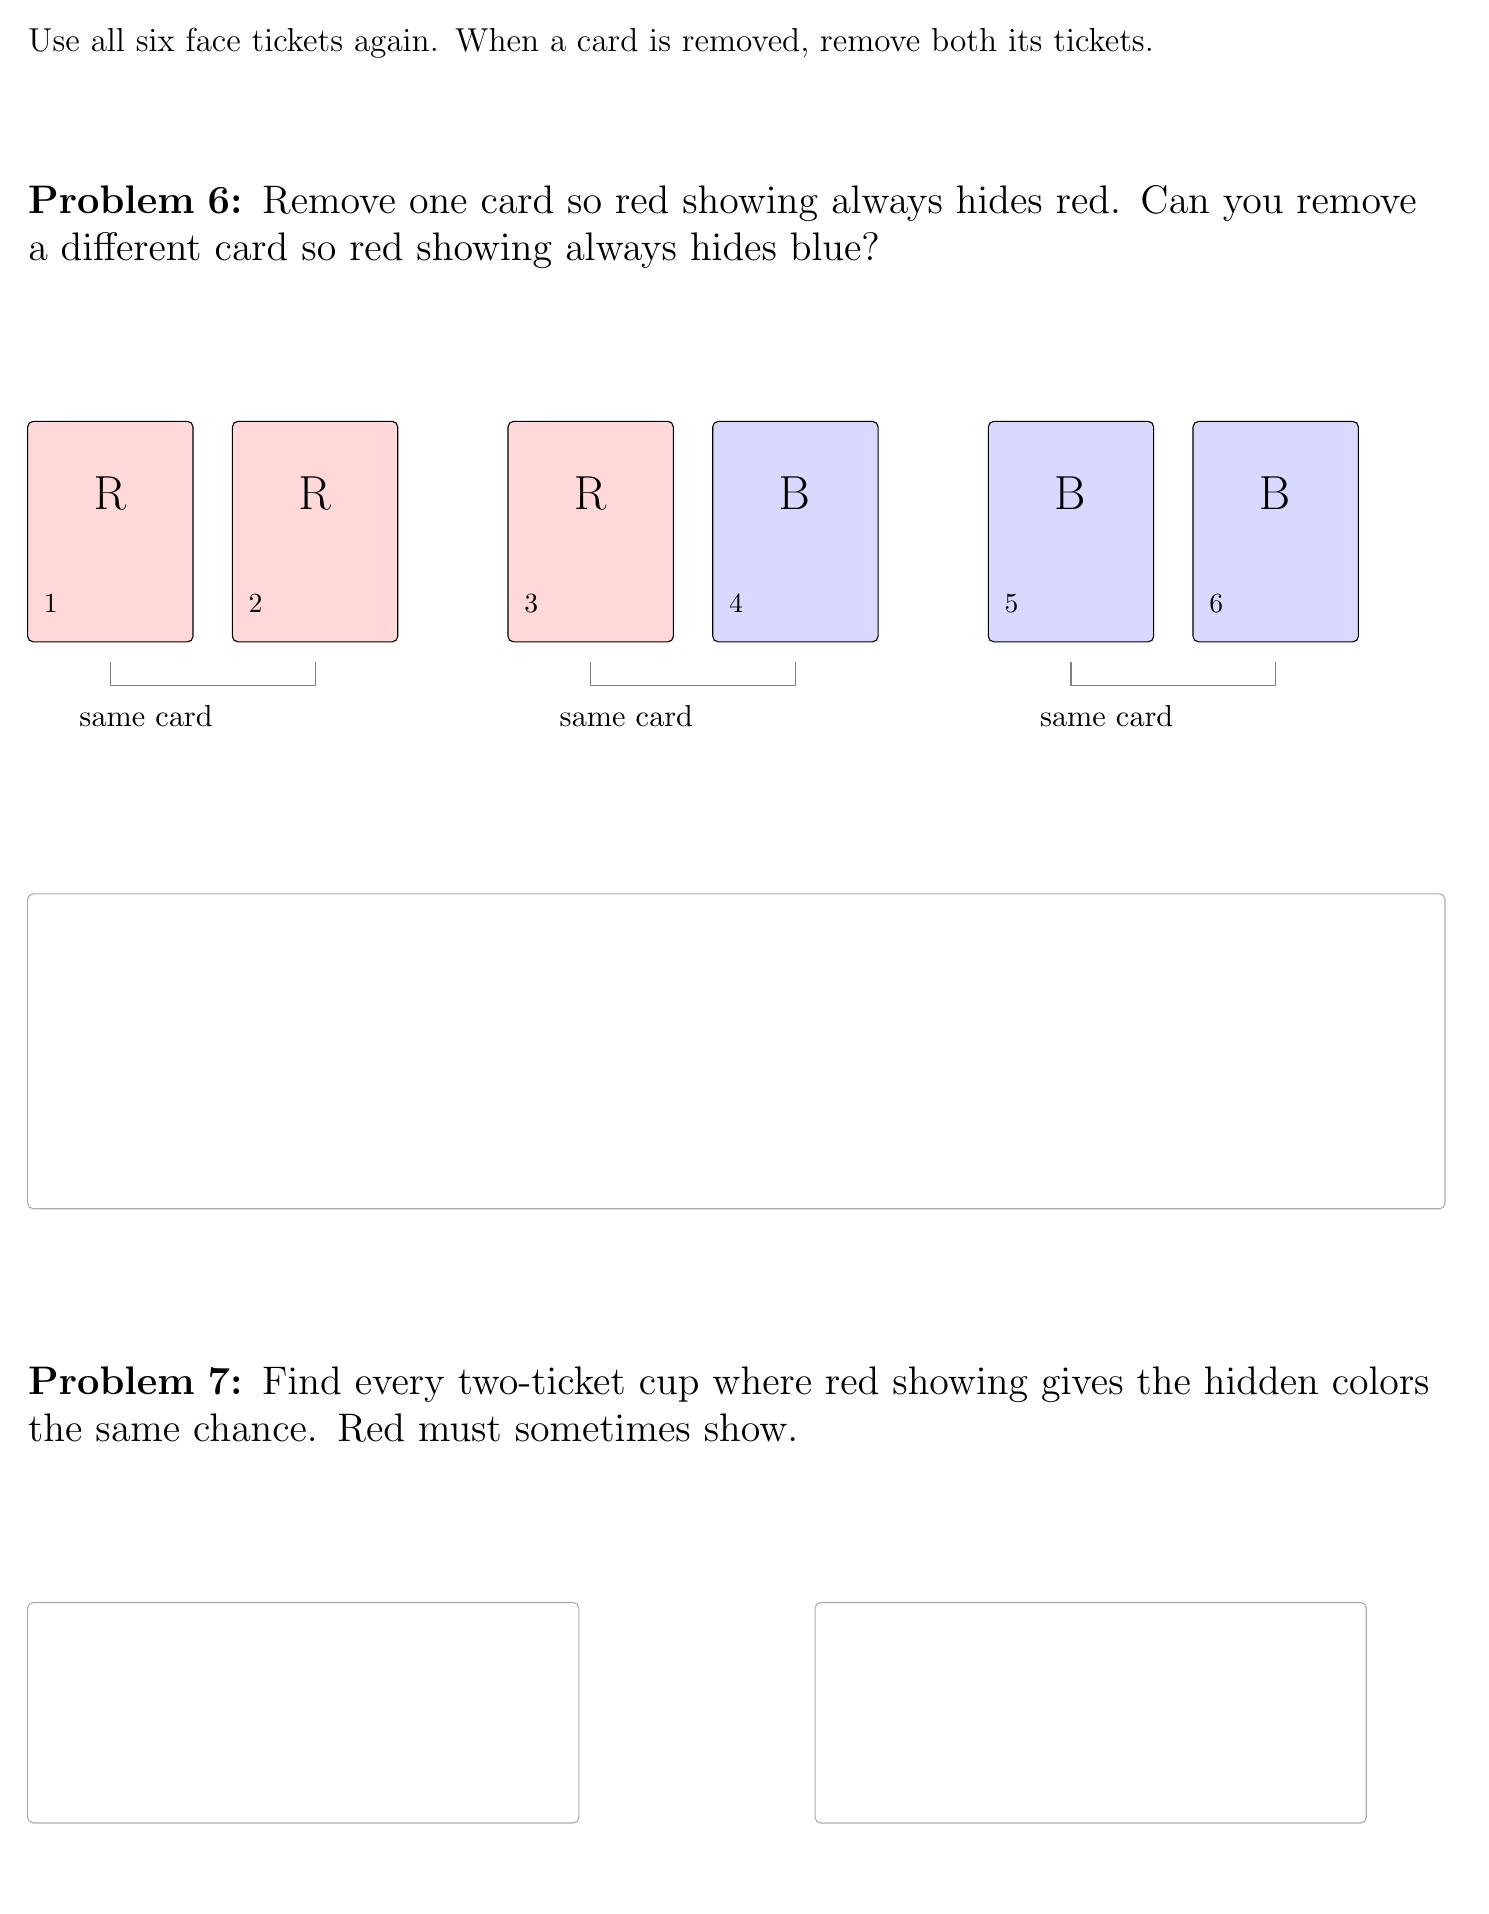
\begin{tikzpicture}[x=1cm,y=1cm]\path[use as bounding box] (0,0) rectangle (18.2,-23.6);
\node[anchor=north west,text width=18cm,inner sep=0pt,font=\fontsize{13}{16}\selectfont] at (0,0) {Use all six face tickets again. When a card is removed, remove both its tickets.};
\node[anchor=north west,text width=18cm,inner sep=0pt,font=\fontsize{14}{17}\selectfont] at (0,-2) {\textbf{Problem 6:} Remove one card so red showing always hides red. Can you remove a different card so red showing always hides blue?};
\draw[fill=red!15,rounded corners=2pt] (0.0,-5) rectangle (2.1,-7.8);
\node[anchor=north west,text width=0.6cm,inner sep=0pt,font=\fontsize{17}{20}\selectfont] at (0.8300000000000001,-5.7) {R};
\node[anchor=north west,text width=0.7cm,inner sep=0pt,font=\fontsize{10}{13}\selectfont] at (0.2,-7.2) {1};
\draw[fill=red!15,rounded corners=2pt] (2.6,-5) rectangle (4.7,-7.8);
\node[anchor=north west,text width=0.6cm,inner sep=0pt,font=\fontsize{17}{20}\selectfont] at (3.43,-5.7) {R};
\node[anchor=north west,text width=0.7cm,inner sep=0pt,font=\fontsize{10}{13}\selectfont] at (2.8000000000000003,-7.2) {2};
\draw[gray] (1.05,-8.05) -- (1.05,-8.35) -- (3.65,-8.35) -- (3.65,-8.05);
\node[anchor=north west,text width=4cm,inner sep=0pt,font=\fontsize{11}{14}\selectfont] at (0.65,-8.6) {same card};
\draw[fill=red!15,rounded corners=2pt] (6.1,-5) rectangle (8.2,-7.8);
\node[anchor=north west,text width=0.6cm,inner sep=0pt,font=\fontsize{17}{20}\selectfont] at (6.93,-5.7) {R};
\node[anchor=north west,text width=0.7cm,inner sep=0pt,font=\fontsize{10}{13}\selectfont] at (6.3,-7.2) {3};
\draw[fill=blue!15,rounded corners=2pt] (8.7,-5) rectangle (10.799999999999999,-7.8);
\node[anchor=north west,text width=0.6cm,inner sep=0pt,font=\fontsize{17}{20}\selectfont] at (9.53,-5.7) {B};
\node[anchor=north west,text width=0.7cm,inner sep=0pt,font=\fontsize{10}{13}\selectfont] at (8.899999999999999,-7.2) {4};
\draw[gray] (7.1499999999999995,-8.05) -- (7.1499999999999995,-8.35) -- (9.75,-8.35) -- (9.75,-8.05);
\node[anchor=north west,text width=4cm,inner sep=0pt,font=\fontsize{11}{14}\selectfont] at (6.75,-8.6) {same card};
\draw[fill=blue!15,rounded corners=2pt] (12.2,-5) rectangle (14.299999999999999,-7.8);
\node[anchor=north west,text width=0.6cm,inner sep=0pt,font=\fontsize{17}{20}\selectfont] at (13.03,-5.7) {B};
\node[anchor=north west,text width=0.7cm,inner sep=0pt,font=\fontsize{10}{13}\selectfont] at (12.399999999999999,-7.2) {5};
\draw[fill=blue!15,rounded corners=2pt] (14.799999999999999,-5) rectangle (16.9,-7.8);
\node[anchor=north west,text width=0.6cm,inner sep=0pt,font=\fontsize{17}{20}\selectfont] at (15.629999999999999,-5.7) {B};
\node[anchor=north west,text width=0.7cm,inner sep=0pt,font=\fontsize{10}{13}\selectfont] at (14.999999999999998,-7.2) {6};
\draw[gray] (13.25,-8.05) -- (13.25,-8.35) -- (15.85,-8.35) -- (15.85,-8.05);
\node[anchor=north west,text width=4cm,inner sep=0pt,font=\fontsize{11}{14}\selectfont] at (12.85,-8.6) {same card};
\draw[gray!65,rounded corners=2pt] (0,-11) rectangle (18,-15);
\node[anchor=north west,text width=18cm,inner sep=0pt,font=\fontsize{14}{17}\selectfont] at (0,-17) {\textbf{Problem 7:} Find every two-ticket cup where red showing gives the hidden colors the same chance. Red must sometimes show.};
\draw[gray!65,rounded corners=2pt] (0,-20) rectangle (7,-22.8);
\draw[gray!65,rounded corners=2pt] (10,-20) rectangle (17,-22.8);
\end{tikzpicture}
\end{document}
